% !TeX program = xelatex
\documentclass[11pt,a4paper]{ctexart}
\usepackage[a4paper,margin=1in]{geometry}
\usepackage{amsmath}
\usepackage{booktabs}
\usepackage{graphicx}
\usepackage{float}
\usepackage{hyperref}
\usepackage{enumitem}
\usepackage{caption}

\title{如果换一种问法，LLM 排名会改变吗？\\
\large 基于非语义 Prompt 扰动与子集重采样的排名逆转分析}
\author{ST5230 Group 14\\
ZHANG QIANCHI \and PENG YANGYUNZHI \and JIANG YIFAN \and MENG XIANGCHEN}
\date{}

\begin{document}
\maketitle

\begin{abstract}
静态 leaderboard 默认假设模型排名在合理的评测设定变化下保持稳定。本文检验这一假设。我们研究非语义 prompt 扰动与评测子集变化是否足以改变三个多项选择 benchmark 上的模型排名：MMLU、ARC-Challenge 与 HellaSwag。我们构建了 900 道题目，将其扩展为 3,600 条 prompt request，并收集 GPT-4o-mini、Gemini-2.0-flash、Qwen-2.5-7B 和 Llama-3.1-8B 的 14,400 条响应。我们对所有输出进行自动评分，并在每个数据集上进行 2,000 次 bootstrap 重采样，以估计置信区间、成对显著性和 ranking reversal rate（RRR）。结果表明，排名稳定性高度依赖 benchmark 本身。ARC-Challenge 极为稳定，MMLU 中等稳定且不确定性主要集中在中间名次，而 HellaSwag 明显更不稳定，在某一 prompt 变体下的排名逆转率达到 62.55\%。
\end{abstract}

\section{引言}

大语言模型评测通常以 leaderboard 的形式呈现。模型被赋予 benchmark 分数，按准确率排序，再将这个顺序视作模型相对能力的稳定摘要。这种做法方便，但它隐含了一个很强的前提：只要任务本身不变，评测细节上的小变化不应显著改变模型之间的相对排序。

这个前提并不当然成立。即使底层任务保持不变，prompt 措辞、答案格式提醒和指令顺序也可能改变模型的行为；同样，一个 benchmark 分数也依赖于恰好被纳入评测的题目子集。如果模型间的真实差距较小，那么 prompt 噪声或样本组成噪声就可能足以改变“谁排第一”的结论。

因此，本文从\textbf{排名稳定性}而非单纯分数波动的角度研究 leaderboard 的可靠性。我们不仅问 prompt 扰动是否会改变准确率，更问一个更严格的问题：这些变化是否已经大到足以改变模型之间的相对排序？

本文的贡献主要有三点：
\begin{enumerate}[leftmargin=1.5em]
\item 我们不只使用单一 benchmark prompt，而是在四类 task-preserving prompt 下分析排名稳定性。
\item 我们将 prompt 扰动与 bootstrap 子集重采样结合起来，同时量化 prompt 噪声与样本组成噪声。
\item 我们不仅报告平均准确率和置信区间，还显式报告 ranking reversal rate、rank probability 和成对显著性，从而直接刻画排序稳健性。
\end{enumerate}

\section{相关工作视角}

本文与三类已有研究密切相关。第一类是 benchmark 构建工作。MMLU、ARC 和 HellaSwag 分别代表多学科知识、多步推理以及常识续写等不同类型的评测场景。第二类是 prompt 鲁棒性研究，相关工作表明模型对 prompt 形式具有显著敏感性。第三类是评测可靠性讨论，即评测结果不仅是模型本身的属性，也受到协议设计、样本选择和实现细节的影响。本文在这一视角上进一步推进，重点关注这些扰动是否会改变模型排序结构。

\section{实验设计}

\subsection{数据集与抽样}

我们使用三个可自动评分的四选一 benchmark：
\begin{itemize}[leftmargin=1.5em]
\item \textbf{MMLU}：共 300 题，从 6 个 subject 中各抽取 50 题。
\item \textbf{ARC-Challenge}：从官方 test split 抽取 300 题。
\item \textbf{HellaSwag}：从 validation split 抽取 300 题，因为公开 test split 不提供 gold label。
\end{itemize}
这样得到总计 900 道题目的 master sample。

\subsection{Prompt 模板}

对每道题，我们构造四类 task-preserving prompt：
\texttt{minimal\_instruction}、\texttt{benchmark\_style}、\texttt{natural\_style} 和 \texttt{order\_phrasing\_variation}。这些模板保持任务语义与答案集合不变，只改变呈现风格、指令口吻和信息顺序。900 道题在 4 个模板下扩展为 3,600 条 prompt request。

\subsection{模型与推理}

我们评测四个模型：
\begin{itemize}[leftmargin=1.5em]
\item \texttt{openai/gpt-4o-mini}
\item \texttt{google/gemini-2.0-flash-001}
\item \texttt{qwen/qwen-2.5-7b-instruct}
\item \texttt{meta-llama/llama-3.1-8b-instruct}
\end{itemize}

将 4 个模型应用于 3,600 条 prompt request，共得到 14,400 条模型响应。所有响应通过 OpenRouter 生成，推理参数为 \texttt{temperature = 0} 和 \texttt{max\_tokens = 150}。14,400 条响应中只有 3 条解析失败，占比 0.02\%，且全部来自 Llama 的安全拒答。

\subsection{Bootstrap 与 RRR}

对每个数据集，我们进行 2,000 次 bootstrap 重采样。每次迭代都从该数据集对应题目中有放回抽样，并重新计算 prompt-specific accuracy、prompt-averaged accuracy、模型间成对差值以及各 prompt 下的模型排序。95\% 置信区间由 bootstrap 分布的 2.5\% 和 97.5\% 分位数构造。

我们将 \texttt{minimal\_instruction} 作为 baseline prompt。对每次 bootstrap 迭代，我们比较其他 prompt 下的模型排序与 baseline 排序；只要顺序发生任何变化，就记为一次 ranking reversal。Ranking Reversal Rate（RRR）即发生 reversal 的迭代比例。

\section{主要结果}

\subsection{Prompt-averaged Accuracy}

\begin{table}[H]
\centering
\caption{Prompt-averaged accuracy 及 95\% 置信区间。}
\begin{tabular}{llccc}
\toprule
数据集 & 模型 & 准确率 & 95\% CI & 排名 \\
\midrule
ARC-Challenge & Gemini-2.0-flash & 94.00\% & [91.42, 96.50] & 1 \\
ARC-Challenge & GPT-4o-mini & 90.83\% & [87.58, 93.75] & 2 \\
ARC-Challenge & Qwen-2.5-7B & 85.08\% & [81.17, 88.92] & 3 \\
ARC-Challenge & Llama-3.1-8B & 77.33\% & [73.25, 82.00] & 4 \\
HellaSwag & GPT-4o-mini & 89.17\% & [86.00, 92.09] & 1 \\
HellaSwag & Gemini-2.0-flash & 87.25\% & [84.08, 90.25] & 2 \\
HellaSwag & Qwen-2.5-7B & 84.25\% & [80.83, 87.75] & 3 \\
HellaSwag & Llama-3.1-8B & 68.33\% & [63.92, 72.75] & 4 \\
MMLU & Gemini-2.0-flash & 85.08\% & [81.17, 88.58] & 1 \\
MMLU & GPT-4o-mini & 73.42\% & [68.67, 78.17] & 2 \\
MMLU & Qwen-2.5-7B & 70.33\% & [65.58, 75.17] & 3 \\
MMLU & Llama-3.1-8B & 60.08\% & [55.08, 65.25] & 4 \\
\bottomrule
\end{tabular}
\end{table}

从点估计上看，Gemini 在 ARC-Challenge 和 MMLU 上领先，而 GPT-4o-mini 在 HellaSwag 上领先。但这些“第一名”结论的稳固程度在不同 benchmark 上并不相同。

\subsection{排名逆转率}

\begin{table}[H]
\centering
\caption{相对于 minimal prompt 的 RRR。}
\begin{tabular}{lccc}
\toprule
数据集 & Benchmark & Natural & Order/Phrasing \\
\midrule
ARC-Challenge & 4.70\% & 1.65\% & 1.05\% \\
HellaSwag & 62.55\% & 41.35\% & 38.50\% \\
MMLU & 19.60\% & 8.05\% & 13.50\% \\
\bottomrule
\end{tabular}
\end{table}

这个结果并不是“小幅且统一”的扰动。ARC-Challenge 极为稳定，MMLU 中等稳定，而 HellaSwag 明显更不稳定，在 benchmark-style prompt 下有超过六成的 bootstrap 迭代发生排名逆转。

\subsection{成对显著性分析}

成对 bootstrap 分析进一步揭示了不确定性集中在哪里：
\begin{itemize}[leftmargin=1.5em]
\item \textbf{ARC-Challenge}：所有成对比较都在 95\% 水平上显著成立。
\item \textbf{HellaSwag}：GPT-4o-mini 相对 Gemini 的差值仅为 1.92\%，95\% CI 为 [-0.67, 4.75]，$p=0.169$。
\item \textbf{HellaSwag}：Gemini 相对 Qwen 的差值为 3.00\%，95\% CI 为 [-0.58, 6.42]，$p=0.102$。
\item \textbf{MMLU}：Gemini 相对 GPT 的差值为 11.67\%，95\% CI 为 [6.99, 16.08]。
\item \textbf{MMLU}：GPT 相对 Qwen 的差值仅为 3.08\%，95\% CI 为 [-1.50, 7.58]，$p=0.184$。
\end{itemize}

\section{分数据集分析}

\subsection{ARC-Challenge：稳定的 leaderboard}

ARC-Challenge 是本研究中最稳定的数据集。Gemini 在所有 prompt 下都保持领先，且所有成对差值都显著。极低的 RRR 说明 prompt 扰动和子集重采样不足以颠覆模型排序。

\subsection{HellaSwag：脆弱的榜首}

HellaSwag 是对“静态 leaderboard 稳定”这一假设最直接的反例。虽然 GPT-4o-mini 的点估计最高，但它相对 Gemini 的优势并不显著；与此同时，HellaSwag 在所有非 baseline prompt 下都呈现最高的 RRR。

\subsection{MMLU：榜首稳定，中游不稳}

MMLU 呈现出一种混合模式。Gemini 明显领先，并在不同 prompt 下都保持第一；但 GPT-4o-mini 与 Qwen 并未显著分开，因此中间名次仍不完全稳定。

\section{MMLU Subject 级分析}

我们进一步对 MMLU 做了 subject-aware bootstrap 分析。pooled 与 stratified 的 full-MMLU bootstrap 都得到相同的总体排序：
\[
\text{Gemini-2.0-flash} > \text{GPT-4o-mini} > \text{Qwen-2.5-7B} > \text{Llama-3.1-8B}.
\]
同时，subject 级别的不稳定性差异很大，平均 RRR 从高中国民经济学的 14.50\% 到哲学的 67.93\% 不等，这说明 ranking stability 不仅依赖 benchmark，也依赖 benchmark 内部的 subject 切片。

\section{讨论与局限性}

本文结果支持三个判断：第一，prompt 敏感性不能只理解为分数波动；第二，单一 prompt 的评测过于狭窄；第三，仅报告准确率置信区间还不够，排序稳健性本身应被报告。

本研究也存在明显局限。我们只评测了三个多项选择 benchmark 和四个模型；我们的 prompt 扰动是浅层且 task-preserving 的，因此只覆盖了 prompt 设计空间中的一个受控子集。

\section{结论}

本文讨论的问题是：如果换一种问法，LLM 排名会改变吗？答案是：会，但不是所有 benchmark 都同样严重。ARC-Challenge 的排行榜高度稳定。MMLU 的榜首稳定，但中游名次仍有不确定性。HellaSwag 对 prompt 和子集变化明显更敏感，其表面上的第一名并未显著领先第二名。因此，更可靠的评测实践应当同时报告“谁平均表现最好”以及“这个排序在 prompt 与样本变化下是否稳健”。

\begin{figure}[H]
\centering
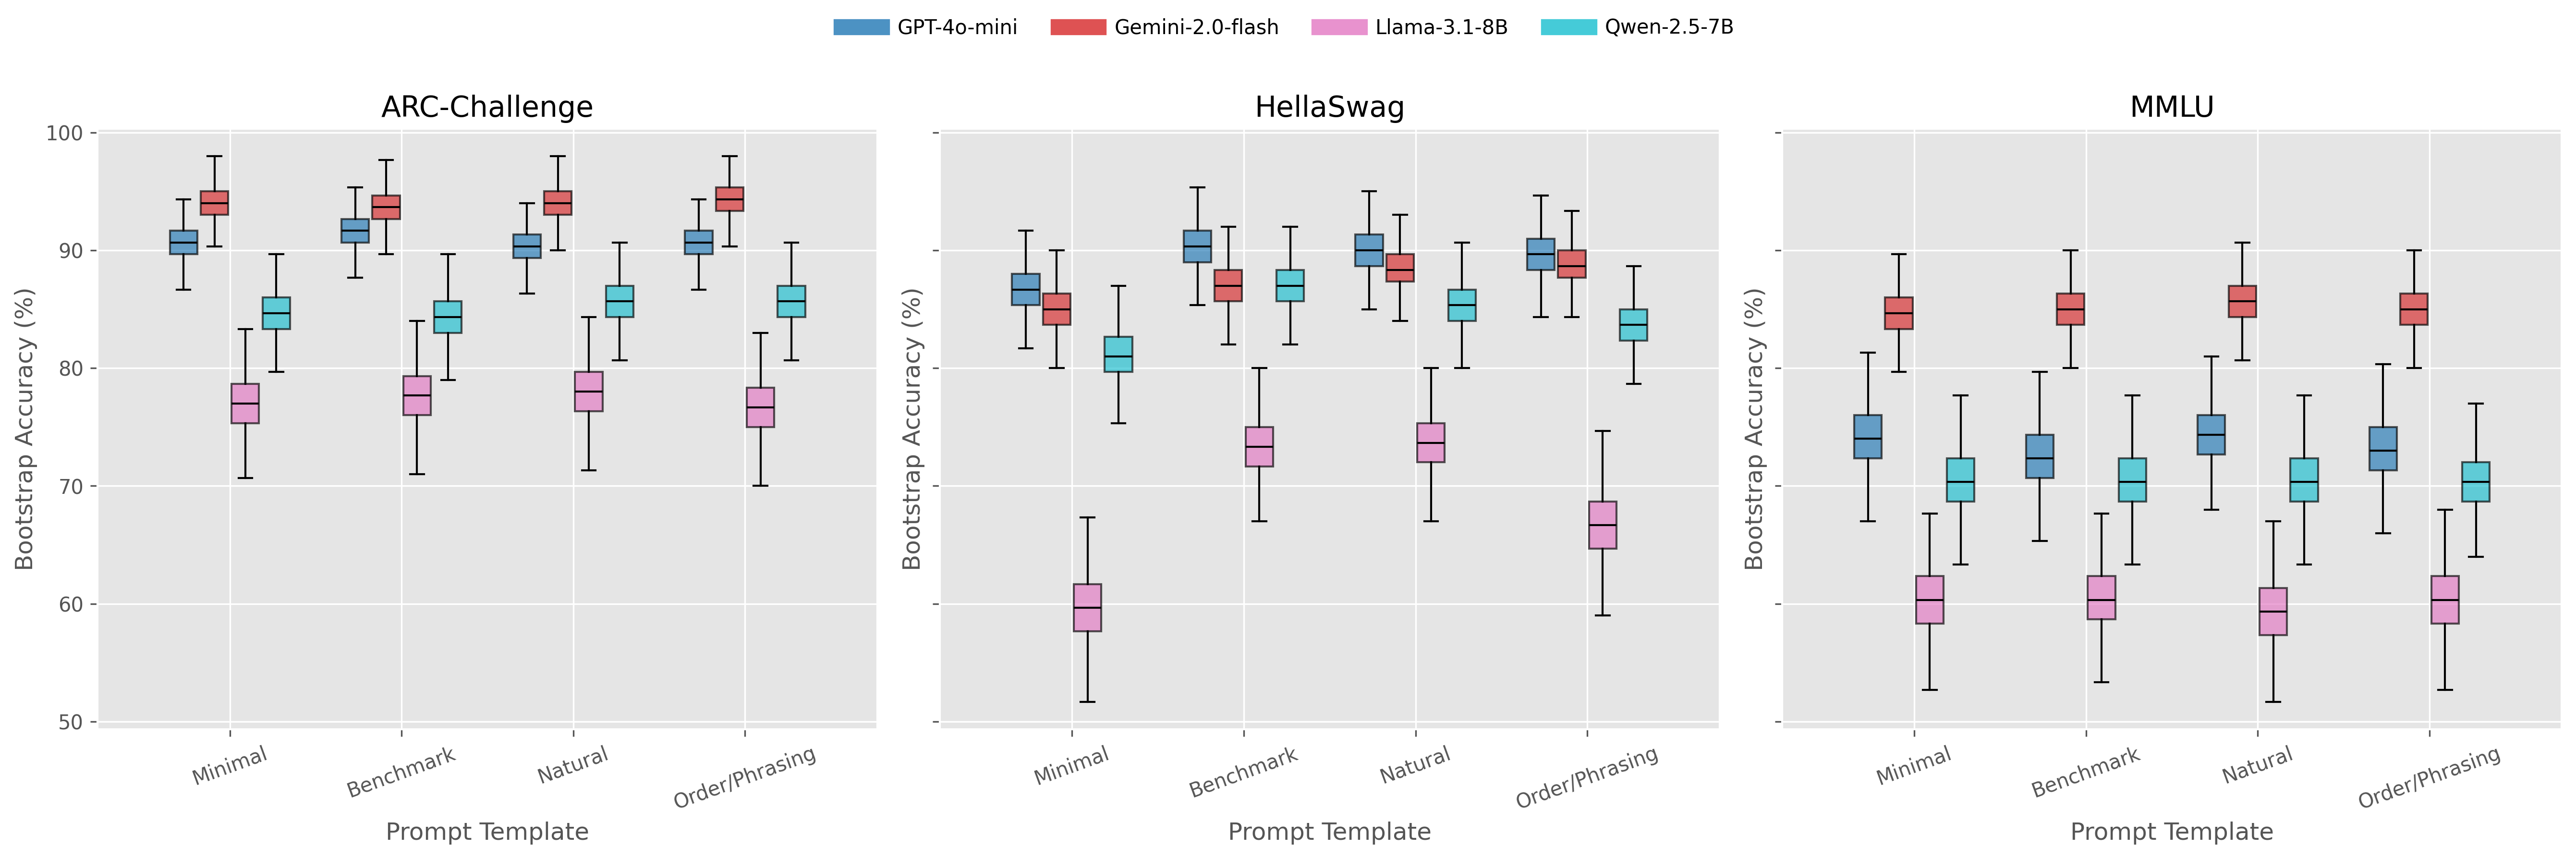
\includegraphics[width=\textwidth]{figures/accuracy_boxplots.png}
\caption{不同 prompt 和数据集下的 bootstrap 准确率箱线图。}
\end{figure}

\begin{figure}[H]
\centering
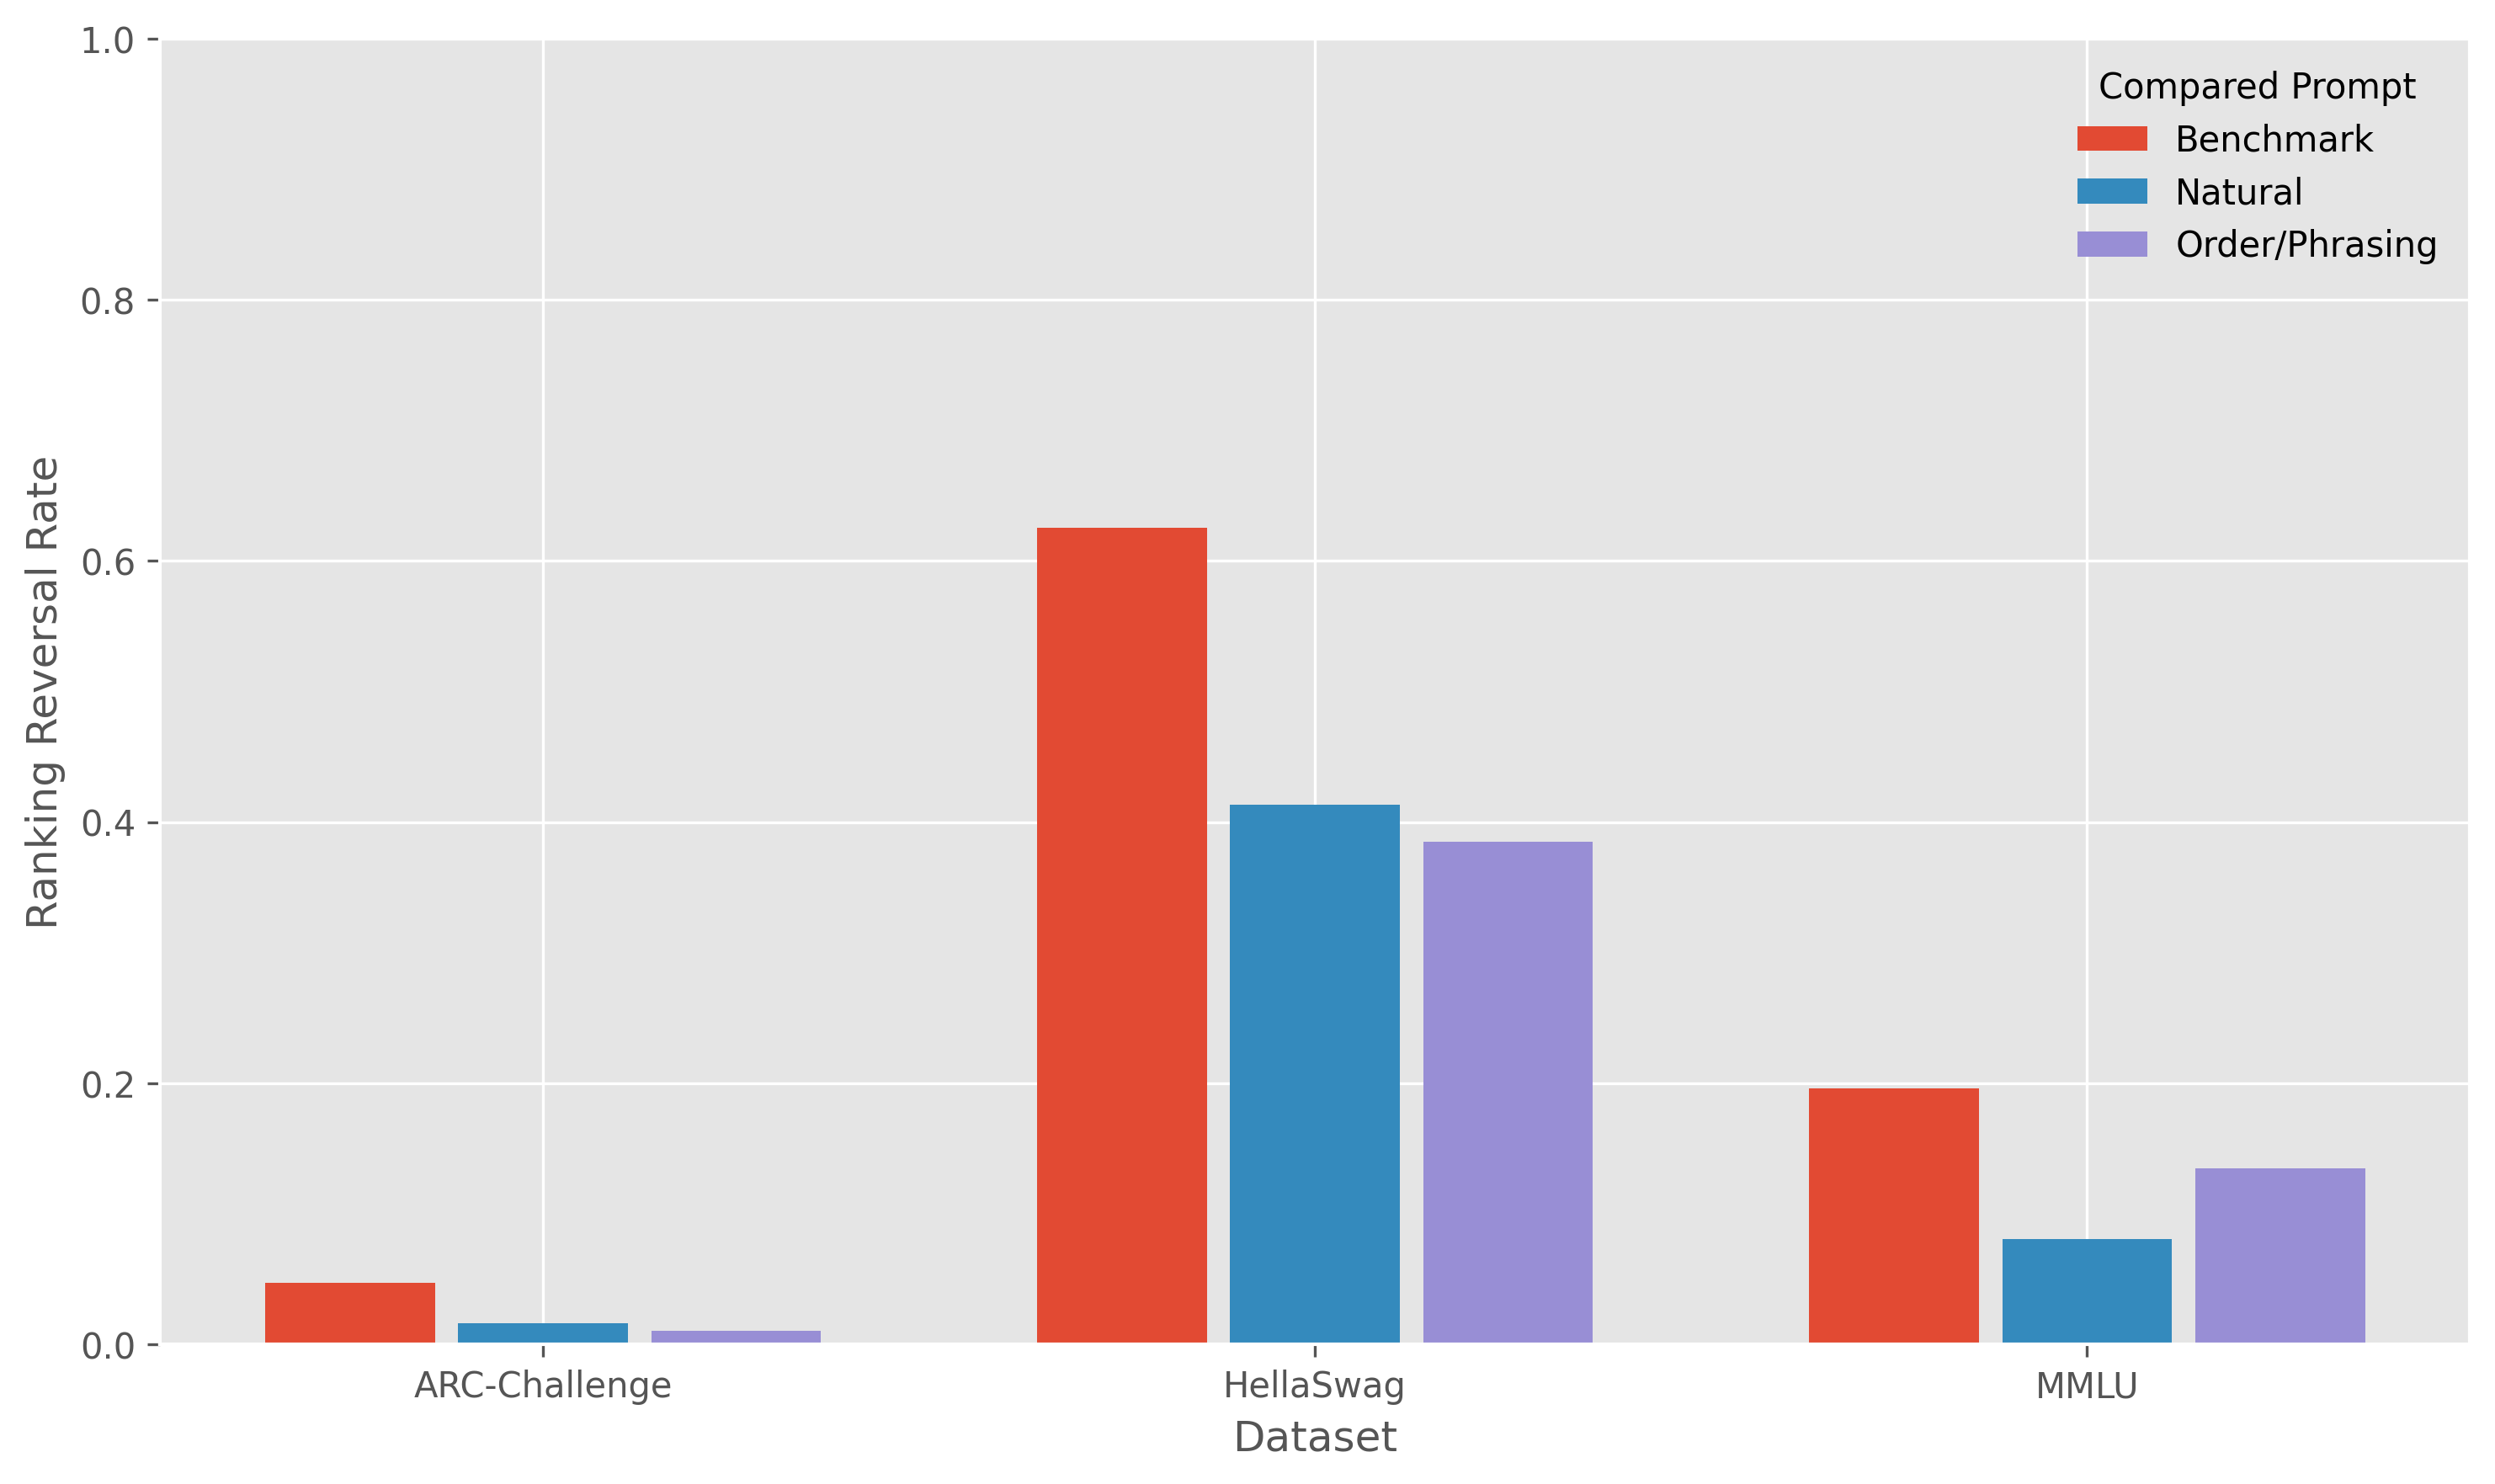
\includegraphics[width=0.72\textwidth]{figures/ranking_reversal_rate.png}
\caption{相对于 minimal prompt 的排名逆转率。}
\end{figure}

\begin{figure}[H]
\centering
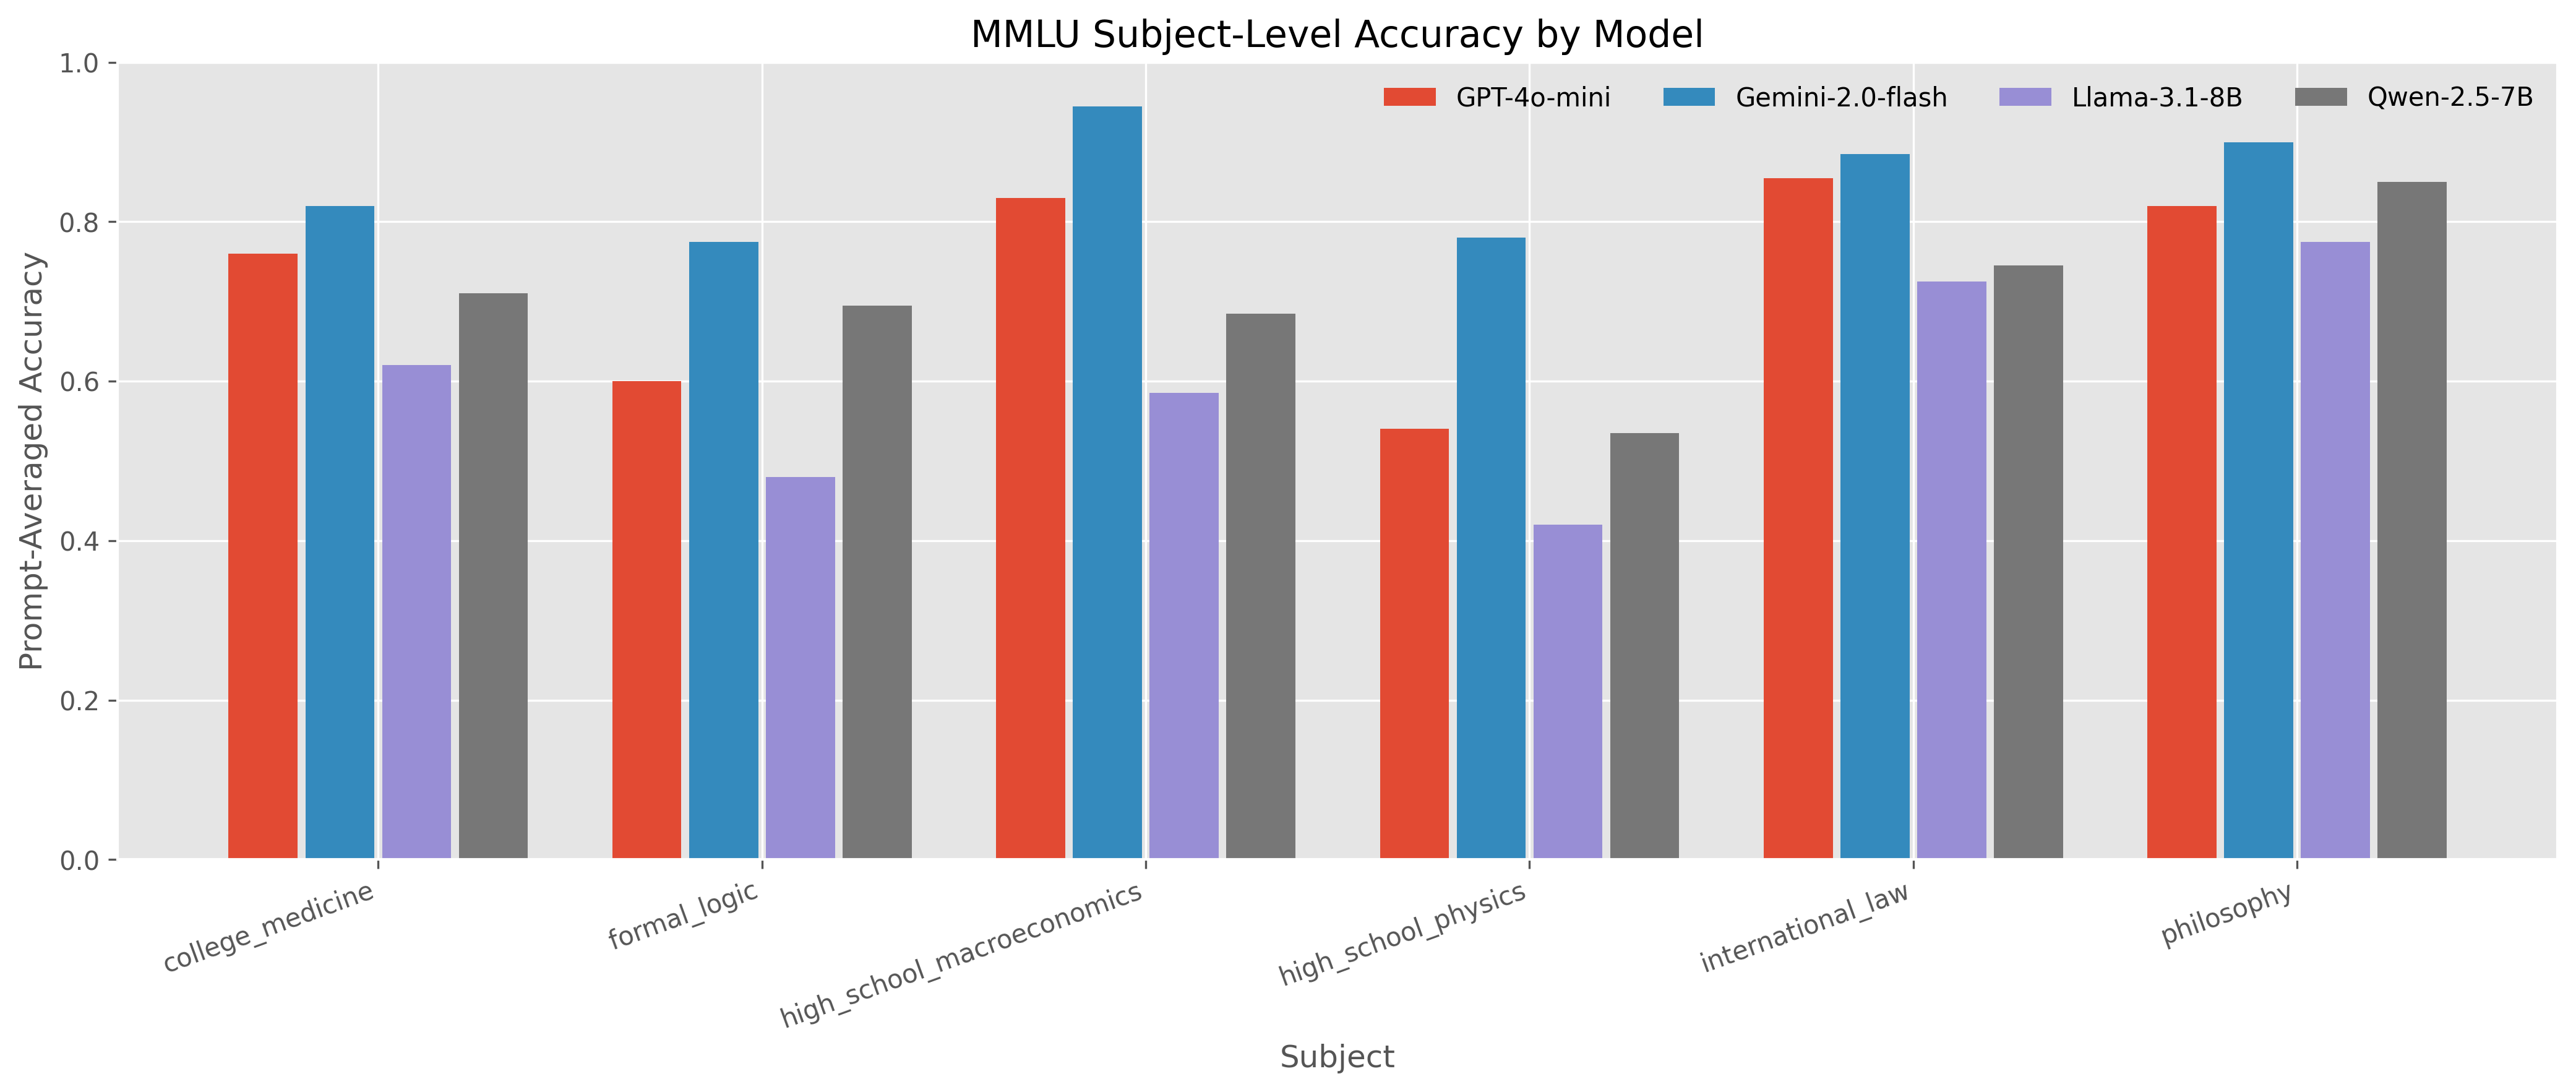
\includegraphics[width=\textwidth]{figures/mmlu_subject_accuracy.png}
\caption{MMLU subject 级别的模型平均准确率。}
\end{figure}

\begin{figure}[H]
\centering
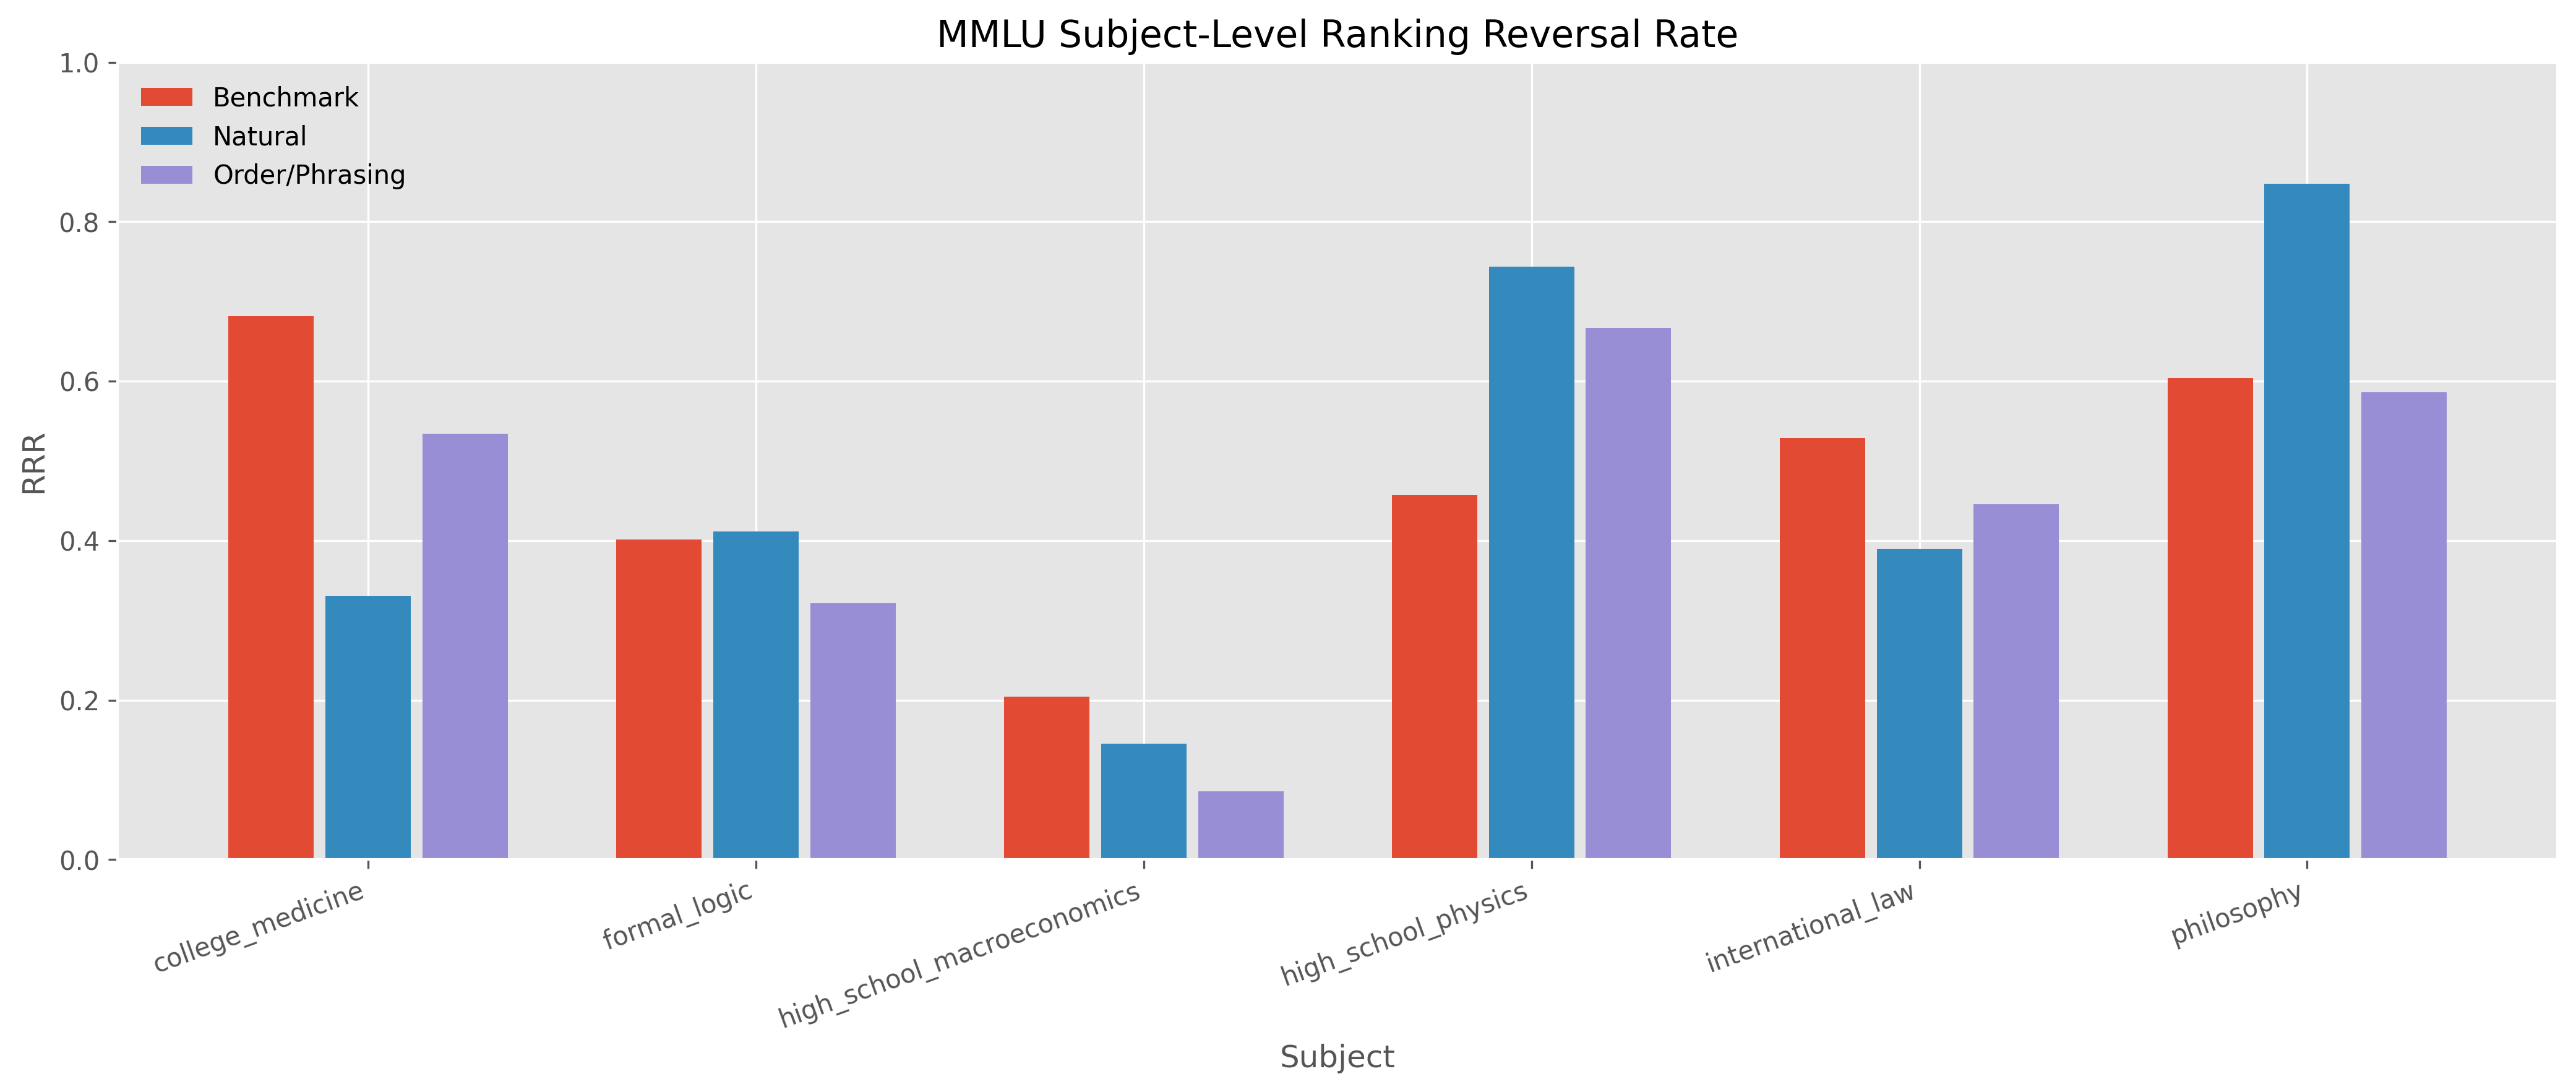
\includegraphics[width=\textwidth]{figures/mmlu_subject_rrr.png}
\caption{MMLU subject 级别的排名逆转率。}
\end{figure}

\begin{thebibliography}{9}
\bibitem{arc}
Clark, P., Cowhey, I., Etzioni, O., Khot, T., Sabharwal, A., Schoenick, C., and Tafjord, O.
\newblock Think You Have Solved Question Answering? Try ARC, the AI2 Reasoning Challenge.
\newblock 2018.

\bibitem{mmlu}
Hendrycks, D., Burns, C., Basart, S., Zou, A., Mazeika, M., Song, D., and Steinhardt, J.
\newblock Measuring Massive Multitask Language Understanding.
\newblock 2020.

\bibitem{hellaswag}
Zellers, R., Holtzman, A., Bisk, Y., Farhadi, A., and Choi, Y.
\newblock HellaSwag: Can a Machine Really Finish Your Sentence?
\newblock 2019.

\bibitem{promptrobust}
Zhu, K., Wang, J., Zhou, J., Wang, Z., Chen, H., Wang, Y., Yang, L., Ye, W., Gong, N. Z., Zhang, Y., and Xie, X.
\newblock PromptRobust: Towards Evaluating the Robustness of Large Language Models on Adversarial Prompts.
\newblock 2023.
\end{thebibliography}

\end{document}
